%
\section{The Fundamental Algorithms within SolverUtils}
\subsection{Filters}
\subsubsection{Lagrangian Points Tracking}
In the filter \texttt{FilterLagrangianPoints}, Lagrangian points can be tracked in parallel. In this filter, Points are stored in two copies. One copy is the stationary points, which are fixed in the thread. Another copy is the mobile points, which can move based on the mesh partition. When evaluating the physics values on the mobile points, we first search the local mesh partition. For the points that are not found in the local partition, their information is packed into a global array and synced for all thread. A global search is performed. Once the thread whose mesh partition contains some unfound mobile points,  these points in the mobile copy are moved to the corresponding thread. After evaluation the physics values on the mobile points, the data are sent back to thread which contains the corresponding stationary points. The design detail of this filter is shown in figure~\ref{fig:LagrangianTrack}.
\begin{figure}[htp]
    \centering
    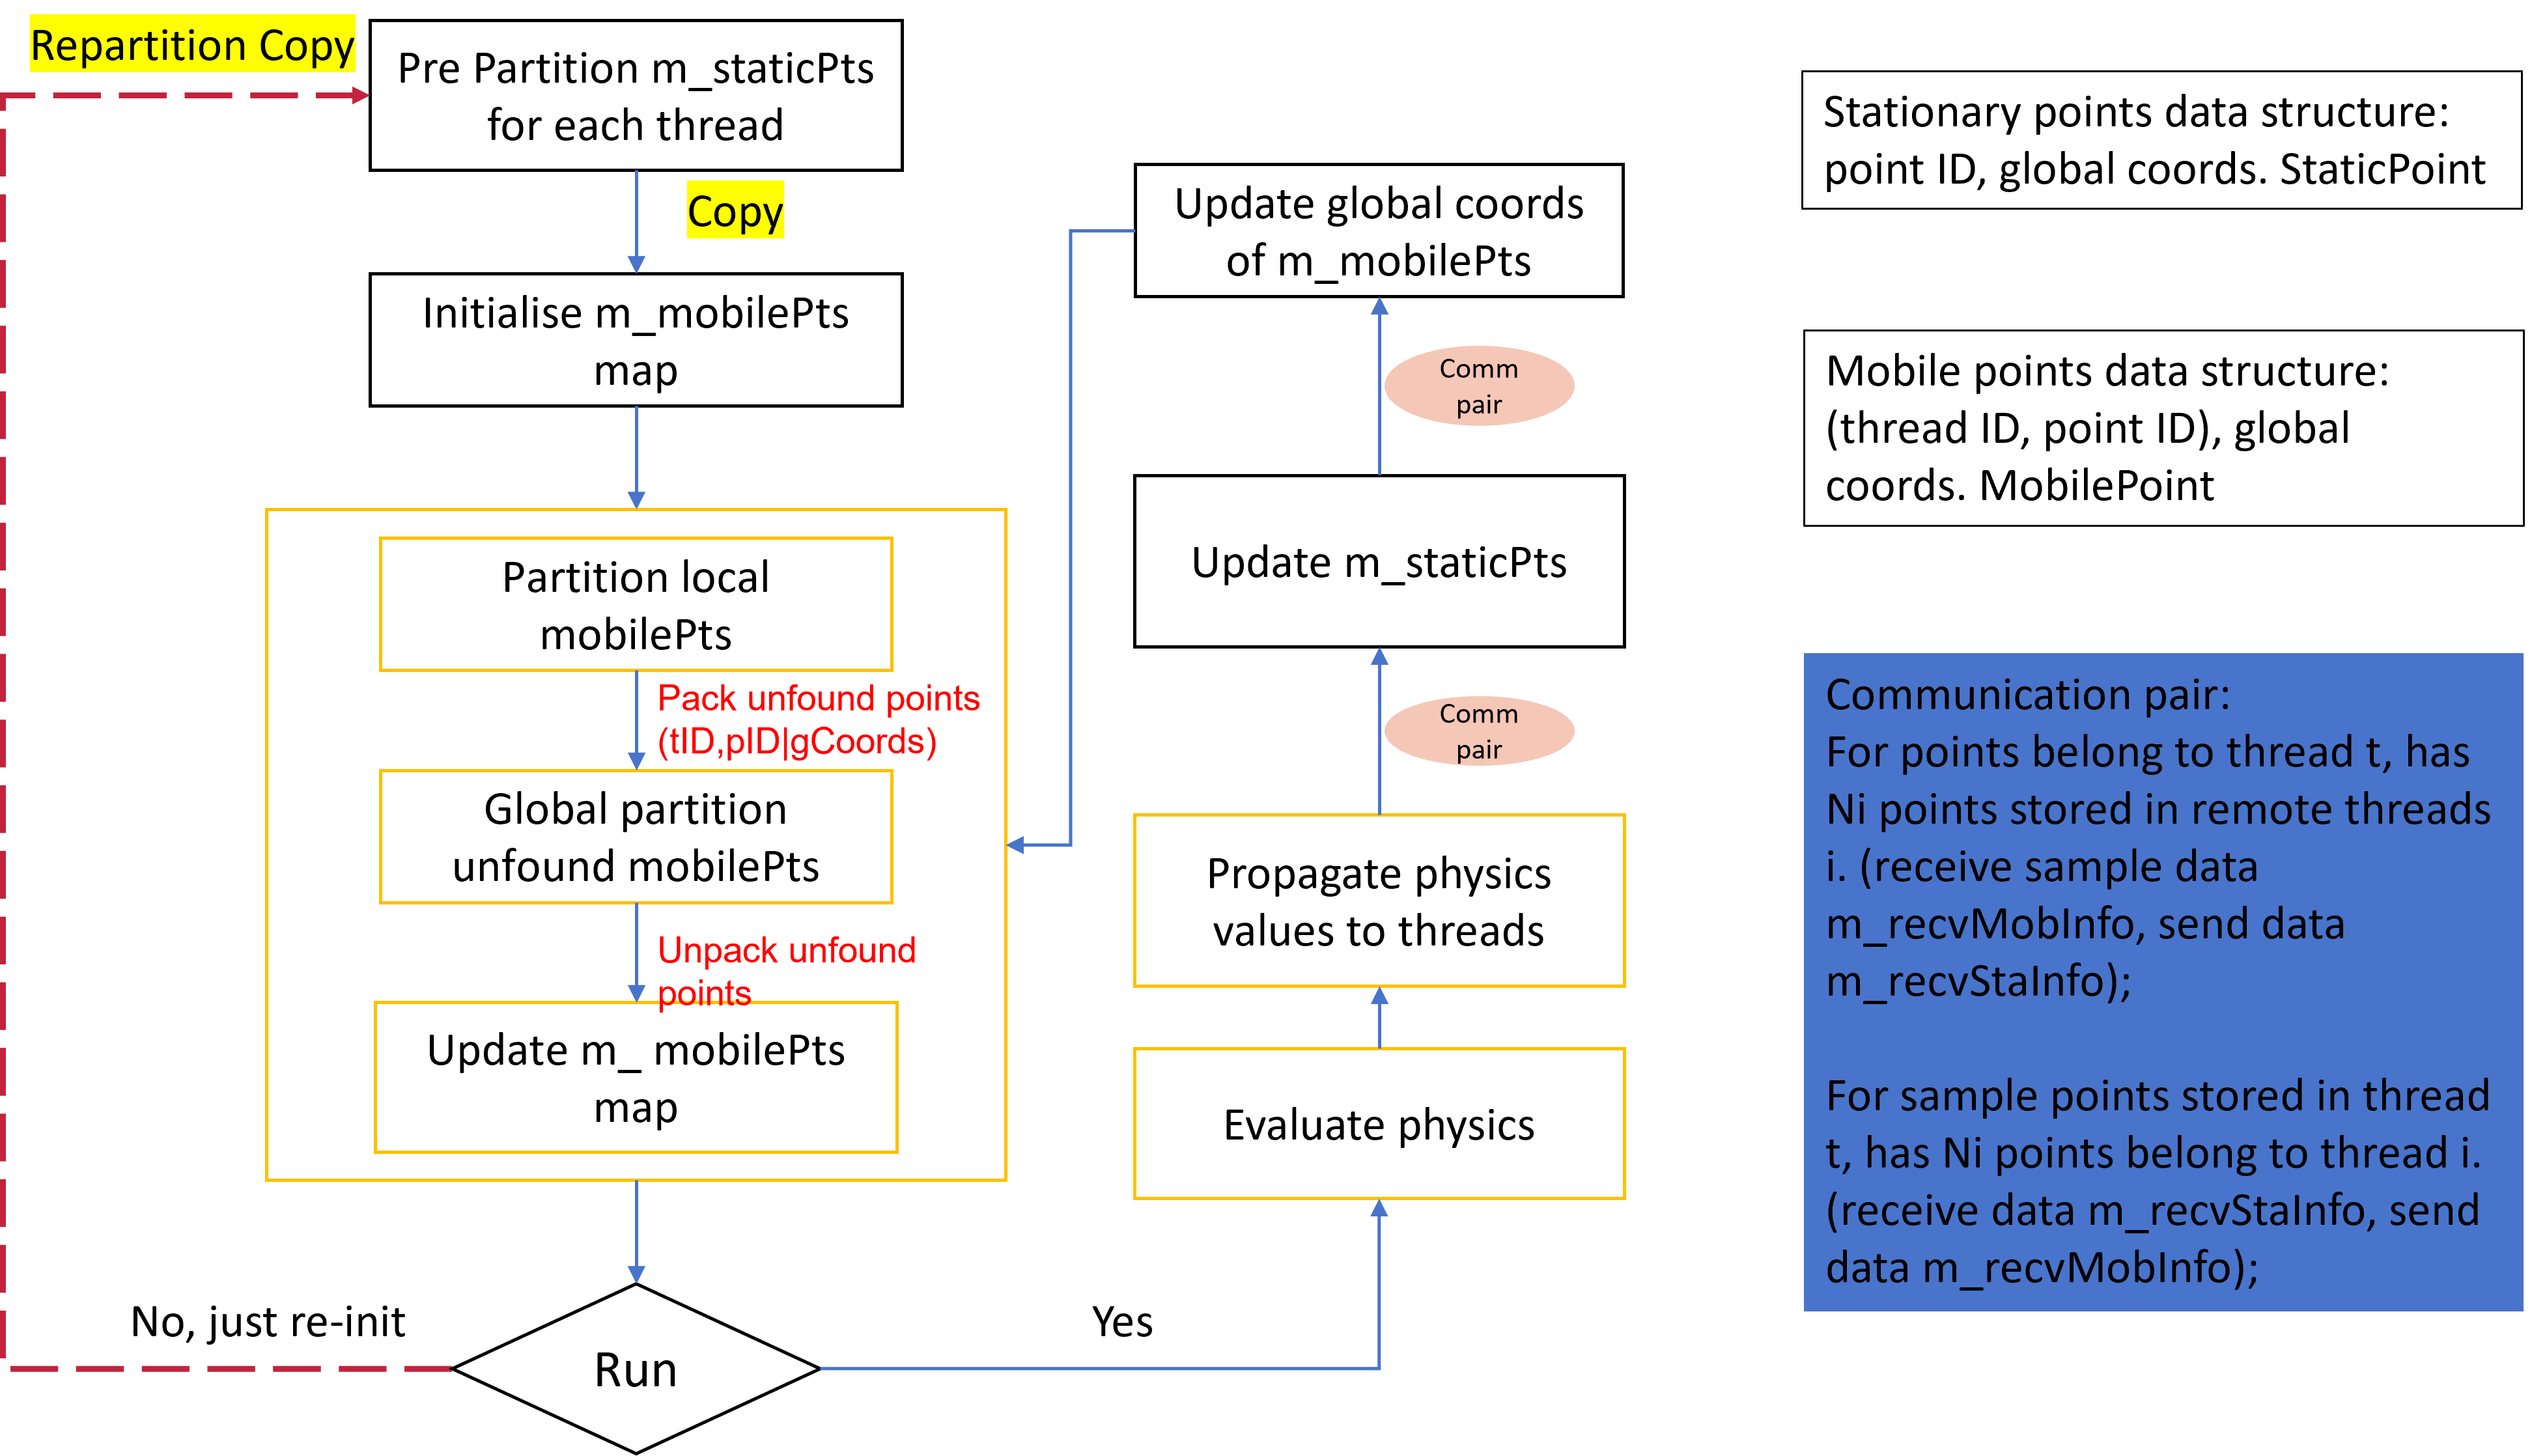
\includegraphics[width=\linewidth]{library/SolverUtils/img/LagrangianPtsTracking.png}
    \label{fig:LagrangianTrack}
    \caption{Design of the \texttt{FilterLagrangianPoints} class} 
\end{figure}